\section{Unity 3D : Modélisation des flux}

\paragraph{} \hspace{10mm}
La dernière partie de mon travail sur ce projet porte sur Unity. A terme, un des objectifs du projet Techn'hom Time Machine est d'avoir une application en Réalité Virtuelle permettant de se déplacer dans le Techn'hom. Il semble évident qu'avec le travail que j'ai déjà accompli et la durée de mon stage, je ne suis pas en mesure de pouvoir développer une telle application. C'est pourquoi dans un premier temps, il a été décidé de créer une application en 3D permettant de visualiser les flux que les données saisies nous ont renseignés. Ici aussi, le manque de temps et mon inexpérience sur Unity font que je ne suis pas en mesure de faire une application complète avec une interface permettant de choisir quel flux afficher. Nous avons donc choisi de faire une maquette de cette application qui permettrait de visionner un seul flux.

\subsection{Schématisation de l'usine}

\paragraph{} \hspace{10mm}
La première partie de notre travail a été la modélisation en 3D du Techn'nom, et plus précisément de l'ancienne usine DMC. Le plus important était d'avoir une carte et des bâtiments parfaitement à l'échelle pour plus de réalisme. Pour ce faire, nous nous sommes appuyés sur un plan de l'usine que Cyril nous a fourni et datant de 1930.

\begin{figure} [H]
    \centering
    \includegraphics[width=1\textwidth]{assets/unity/schema_usine_dmc.jpg}
    \caption{Plan de l'usine DMC}
    \label{fig:planDMC}
\end{figure}

\paragraph{} \hspace{10mm}
Une fois le plan à disposition, nous en avons conclu que la manière la plus simple de modéliser les différents bâtiments à la bonne échelle était simplement de créer un sol dans Unity qui aurait pour texture l'image du plan. Les deux seuls points que nous avons eu à vérifier étaient que l'image ne perde pas ni en qualité ni en résolution lorsqu'on l'appliquerait sur la texture du sol et qu'elle ne se déformerait pas sinon quoi tout ceci n'aurait aucun intérêt.

Par la suite, comme l'application n'en est encore qu'au stade de maquette, nous nous sommes contentés de représenter les bâtiments par de simples rectangles blancs, numérotés selon les indications du plan. Ceux ci sont simplement des objets du type primitif \textbf{Cube} intégré à Unity que l'on a positionnés et dimensionnés par tâtonnement par dessus le plan.

\begin{figure} [H]
    \centering
    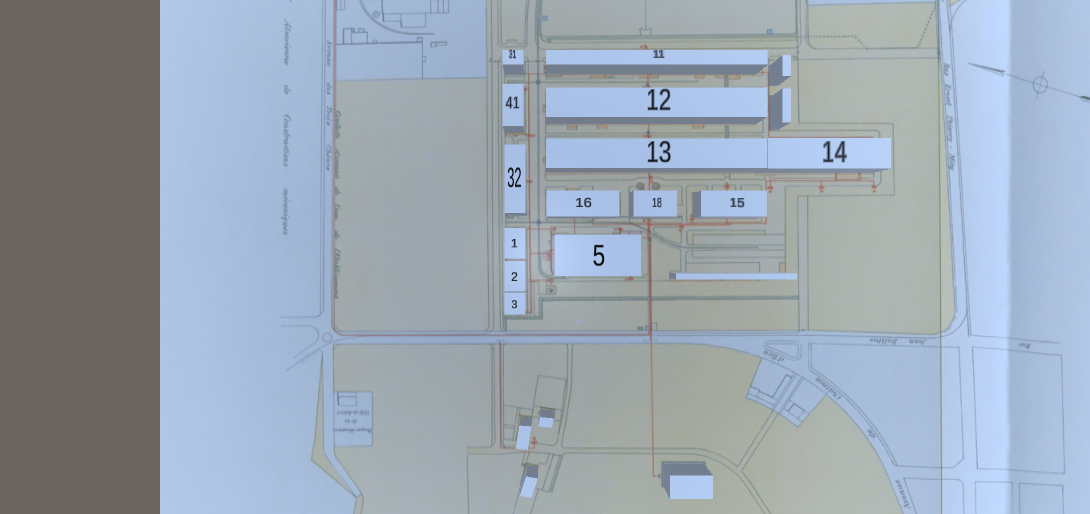
\includegraphics[width=0.79\textwidth]{assets/unity/screen_unity_map.png}
    \caption{Carte de l'application Unity vue du dessus}
    \label{fig:unityMap}
\end{figure}

\subsection{Génération procédurale des flèches}

\paragraph{} \hspace{10mm}
La deuxième partie de notre travail a été de trouver un moyen de faire afficher à l'écran des flèches. Par défaut, Unity ne possède pas ce genre d'objet en type primitif (comme les \textbf{Cube}), il a donc fallu trouver un moyen d'en disposer. La première chose à laquelle nous avons pensé est de trouver un asset sur l'Unity Asset Store. Malheureusement, il n'existe aucun asset gratuit sur le store qui puisse répondre à nos besoins ; seuls certains assets payants étaient intéressants. La deuxième option à laquelle nous avons pensé est le design d'un asset sur Blender. Toutefois, cette option a très vite été écartée car je n'ai aucune connaissance sur Blender, et nous avons donc préféré chercher une autre solution. Enfin, la troisième option à laquelle nous avons réfléchi et que nous avons choisi, est la génération procédurale. La génération procédurale a l'avantage d'être plutôt simple à mettre en oeuvre, et surtout, d'être plus personnalisable qu'un asset pré-fait venant du store.

\begin{figure} [H]
    \centering
    
\includegraphics[width=0.5\textwidth]{assets/unity/screen_fleche2.png}
    \caption{Dessin montrant la flèche générée}
    \label{fig:dessinFleche2}
\end{figure}

\paragraph{} \hspace{10mm}
Pour pouvoir modéliser des flèches, nous avons choisi d'utiliser les \textbf{Mesh} intégrés à Unity. La première étape a été la modélisation de la "queue" : nous avons commencé par générer quatre points pour former un rectangle en partant de l'origine du Mesh, puis nous avons formé deux triangles rectangles dont les hypoténuses se superposent pour former un rectangle. Le positionnement des points dépend de 2 paramètres, ce qui permet de régler la largeur et la longueur de la queue. 

\begin{figure}[H]

\centering

\begin{subfigure}{0.49\textwidth}
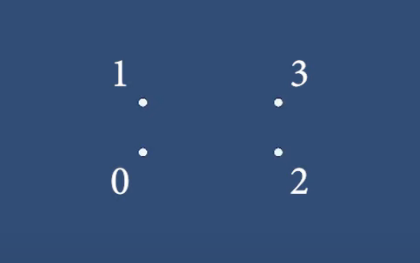
\includegraphics[width=1\linewidth]{assets/unity/screen_point1.png} 
\label{fig:unityPoint1}
\end{subfigure}
\begin{subfigure}{0.49\textwidth}
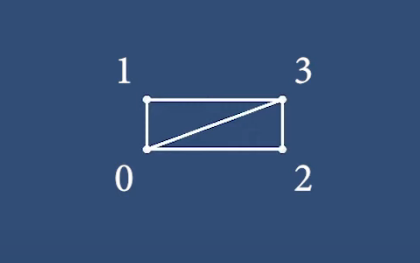
\includegraphics[width=1\linewidth]{assets/unity/screen_point3.png}
\label{fig:unityPoint3}
\end{subfigure}

\caption{Dessins montrant comment est générée la queue de la flèche}
\label{fig:unityPoint1&3}
\end{figure}

\paragraph{} \hspace{10mm}
Enfin, la deuxième partie du travail a été la modélisation de la tête de la flèche. Pour ce faire, nous avons utilisé la même méthode que pour la queue mais en ne plaçant que 3 points pour former un triangle. Ces 3 points sont placés en bout de queue et dépendent eux aussi de deux paramètres afin de pouvoir changer la longueur et la largeur de la tête de la flèche.

\begin{figure}[H]

\centering

\begin{subfigure}{0.49\textwidth}
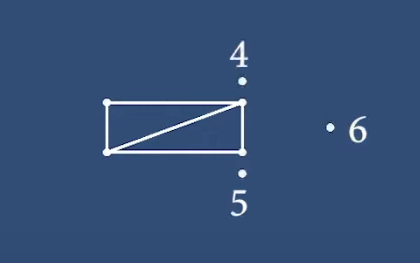
\includegraphics[width=1\linewidth]{assets/unity/screen_point2.png} 
\label{fig:unityPoint2}
\end{subfigure}
\begin{subfigure}{0.49\textwidth}
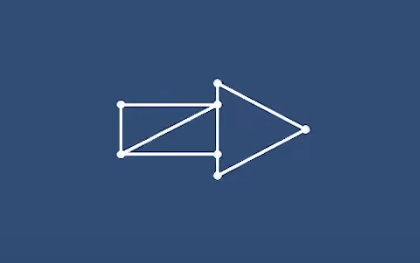
\includegraphics[width=1\linewidth]{assets/unity/screen_fleche1.png}
\label{fig:dessinFleche1}
\end{subfigure}

\caption{Dessins montrant comment est générée la tête de la flèche}
\label{fig:unityPoint2&Fleche1}
\end{figure}

\subsection{API Omeka-S et Représentation des flux}

\paragraph{} \hspace{10mm}
Après avoir fini de préparer tout ce qui concerne la partie graphique, nous avons commencé à travailler avec l'API d'Omeka-S. Cette dernière est plutôt simple à utiliser car elle n'est pas très complexe et surtout très bien documentée\footnote{Lien vers la documentation : \hyperlink{https://omeka.org/s/docs/developer/}{https://omeka.org/s/docs/developer/}}. 

\paragraph{} \hspace{10mm}
Pour pouvoir avoir des données exploitables, la première étape a été de dé-sérialiser les données au format JSON venant de l'API. Cette étape nous a posé quelques problèmes car la structure JSON des items d'Omeka est très irrégulière (les données sont toutes dans un tableau JSON dont les index ont des structures différentes), et dé-sérialiser à la main devient impossible dès lors que l'on a ne serait-ce que quelques items à gérer. Afin de ne pas rester bloqués, nous nous sommes tournés vers Anne Wartelle que nous avions rencontrée à Nantes et qui avait déjà travaillé avec une combinaison d'ontologie et d'Unity. Cette dernière nous a ainsi proposé d'utiliser \hyperlink{https://quicktype.io/}{Quicktype.io} : le site permet d'obtenir du code dé-sérialisant des données au format JSON dans le langage que l'on souhaite. Nous avons donc copié toutes les données de l'API directement depuis le navigateur et nous avons tout collé dans Quicktype. Le principal avantage de cette méthode est sa rapidité : en seulement 1 minute, nous avons eu à disposition du code tout prêt et parfaitement fonctionnel pour tout dé-sérialiser. En revanche, cette méthode comporte aussi un inconvénient : à chaque ajout d'item dans Omeka, notre script Unity devient incapable de gérer les données et nous sommes obligés de re-générer le code pour remplacer l'ancien.

\paragraph{} \hspace{10mm}
Ensuite, la deuxième étape a été de réfléchir à comment traiter les données et comment les exploiter pour pouvoir faire afficher les flux. Ici aussi, nous avons rencontré des problèmes pour trouver une solution durable, maintenable et extensible à cause de la variabilité de la structure des données.

Comme l'application en est encore au stade de maquette et que nous avons décidé de ne modéliser qu'un seul flux, cela simplifie un petit peu les choses : nous n'avons pas besoin de multiplier les requêtes vers le serveur pour obtenir les données voulues à chaque changement de flux à visualiser et l'exploitation est plutôt rapide. La première action à réaliser est d'isoler le flux que nous voulons afficher : pour cela, chaque classe d'objet est identifiée par un entier unique. Dans notre cas, les objets de type \textbf{crm:E9 Move} ont pour ID 114. Cet ID est très pratique car il peut être utilisé dans une query string en paramètre de l'URL pour effectuer des requêtes plus précises\footnote{La query string est : resource\_class\_id}.Une fois notre flux isolé, deux possibilités s'offrent à nous : soit le flux est composé de sous-flux, soit c'est un flux simple. Dans le cas d'un flux simple, il suffit de regarder quels sont le lieu de départ et le lieu d'arrivée du flux. Dans le cas du flux composé, il faut traiter chaque sous-flux un par en suivant le même procédé que pour les flux simples.

Enfin, une fois que nous avons su comment exploiter les données, nous avons réfléchi à comment gérer l'affichage. La solution que nous avons retenu est la suivante : nous pré-disposons des flèches qui vont de bâtiments en bâtiments (pour tous et dans les deux sens) que nous désactivons par défaut. Ensuite, à l'aide des données que l'on vient d'analyser, on détermine à l'aide de booléens quels sont les points de départs et d'arrivées\footnote{Les deux propriétés situant le flux étant distinctes, on connaît la cardinalité d'un flux}. Enfin, selon les booléens qui ont pour valeur \textbf{true}, on peut réactiver les flèches dont on a besoin.

\begin{figure} [H]
    \centering
    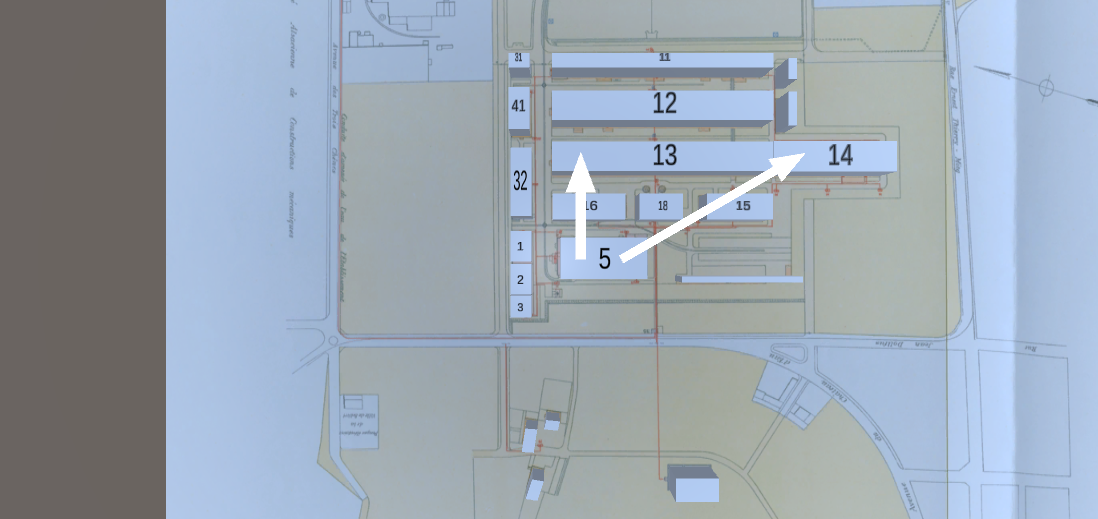
\includegraphics[width=1\textwidth]{assets/unity/screen_unity_flux.png}
    \caption{Modélisation d'un flux vu du dessus}
    \label{fig:unityFlux}
\end{figure}

% Expliquer comment on modélise les flux
